\documentclass[11pt]{article}

\usepackage[margin=1in]{geometry}
\usepackage{amsmath,amssymb,amsthm}
\usepackage{booktabs}
\usepackage{xcolor}
\usepackage{listings}
\usepackage{hyperref}
\usepackage{tikz}
\usetikzlibrary{arrows.meta,positioning,shapes.geometric,calc,fit,backgrounds}

\hypersetup{colorlinks=true,linkcolor=blue!60!black,urlcolor=teal}

% ---- palette / node styles ------------------------------------------------
\definecolor{cproc}{HTML}{1F4E79}
\definecolor{cfill}{HTML}{E8F0FA}
\definecolor{cio}{HTML}{FBEEDC}
\definecolor{cdec}{HTML}{F6D8C8}
\definecolor{cfile}{HTML}{EAF3EA}
\tikzset{
  proc/.style={rectangle, rounded corners=2pt, draw=cproc, thick, fill=cfill,
    align=center, minimum height=9mm, inner sep=4pt, font=\small},
  io/.style={trapezium, trapezium left angle=70, trapezium right angle=110,
    draw=cproc!70, fill=cio, align=center, minimum height=8mm, font=\small},
  dec/.style={diamond, aspect=2.2, draw=cproc!70, fill=cdec, align=center,
    inner sep=1pt, font=\small},
  file/.style={rectangle, draw=green!35!black, fill=cfile, rounded corners=1pt,
    font=\ttfamily\footnotesize, align=center, minimum height=7mm, inner sep=3pt},
  arr/.style={-{Latex[length=2.4mm]}, thick, draw=cproc!85},
  darr/.style={-{Latex[length=2.4mm]}, thick, dashed, draw=gray!70},
}

\lstset{basicstyle=\ttfamily\footnotesize, breaklines=true, columns=fullflexible,
  keywordstyle=\color{cproc}\bfseries, commentstyle=\color{gray}, showstringspaces=false}

\newcommand{\Zq}{\mathbb{Z}_q}
\newcommand{\Rq}{\mathcal{R}_q}
\newcommand{\NTT}{\mathrm{NTT}}
\newcommand{\INTT}{\mathrm{INTT}}
\newcommand{\HtP}{\mathrm{HashToPoint}}

\title{\textbf{Falcon-512 Verification on Starknet}\\[2pt]
\large Implementation Plan, Mathematics, and Optimization}
\author{\texttt{falcon-starknet}}
\date{\today}

\begin{document}
\maketitle

\begin{abstract}
We describe a from-scratch implementation of \textbf{Falcon-512} (NIST FN-DSA) signature
\emph{verification} for Starknet/Cairo. Signing and key generation use floating-point Gaussian
sampling and remain off-chain; only verification---which is integer-only---runs on-chain. We
give the mathematics of each stage (modular arithmetic, the negacyclic number-theoretic
transform, SHAKE-256 hash-to-point, signature/key decoding, and the norm-bounded acceptance
test), the data flow between modules, the code-generation pipeline that emits an unrolled NTT,
and the optimization work (lazy modular reduction, the felt-shift trick, and the compiler
limits that shape the design). All figures are drawn with Ti\emph{k}Z.
\end{abstract}

\tableofcontents

% ===========================================================================
\section{Overview and repository layout}
The system is a vertical of independently validated layers. A Rust \emph{reference}
(Pornin's public-domain \texttt{fn-dsa}) generates genuine signatures and known-answer
fixtures; a Rust \emph{code generator} emits an unrolled Cairo NTT; and the Cairo
\emph{verifier} consumes the fixtures. Figure~\ref{fig:files} shows the module dependencies.

\begin{figure}[h]
\centering
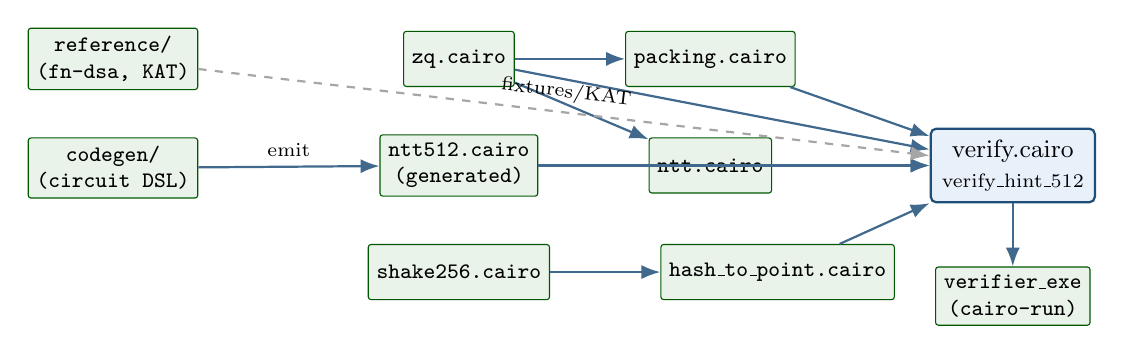
\begin{tikzpicture}[node distance=6mm and 14mm]
  % reference / codegen (rust)
  \node[file] (ref) {reference/\\(fn-dsa, KAT)};
  \node[file, below=of ref] (cg) {codegen/\\(circuit DSL)};
  \node[file, right=26mm of ref] (zq) {zq.cairo};
  \node[file, below=of zq] (nttc) {ntt512.cairo\\(generated)};
  \node[file, below=of nttc] (shake) {shake256.cairo};
  \node[file, right=of zq] (pack) {packing.cairo};
  \node[file, right=of nttc] (ntt) {ntt.cairo};
  \node[file, right=of shake] (h2p) {hash\_to\_point.cairo};
  \node[proc, right=20mm of ntt] (verify) {verify.cairo\\ \scriptsize verify\_hint\_512};
  \node[file, below=8mm of verify] (exe) {verifier\_exe\\(cairo-run)};

  \draw[arr] (cg) -- (nttc) node[midway,above,font=\scriptsize]{emit};
  \draw[arr] (zq) -- (ntt);
  \draw[arr] (zq) -- (pack);
  \draw[arr] (nttc) -- (verify);
  \draw[arr] (ntt) -- (verify);
  \draw[arr] (zq) -- (verify);
  \draw[arr] (pack) -- (verify);
  \draw[arr] (shake) -- (h2p);
  \draw[arr] (h2p) -- (verify);
  \draw[arr] (verify) -- (exe);
  \draw[darr] (ref) -- (verify) node[midway,above,font=\scriptsize,sloped]{fixtures/KAT};
\end{tikzpicture}
\caption{Module dependency flow. Solid: Cairo compile/use edges; dashed: off-chain
fixtures. \texttt{ntt512.cairo} is emitted by the code generator; \texttt{verify.cairo}
composes the transform, ring arithmetic, packing, and the norm test.}
\label{fig:files}
\end{figure}

% ===========================================================================
\section{Mathematical preliminaries}
Falcon operates over the ring
\[
  \Rq = \Zq[x]/(x^{n}+1),\qquad n=512,\quad q=12289=3\cdot 2^{12}+1 .
\]
Since $2n=1024 \mid q-1$, $\Rq$ admits a length-$n$ negacyclic NTT. A key pair is a short
basis of an NTRU lattice; the public key is $h\in\Rq$. A signature of a message $m$ is a pair
of short polynomials $(s_1,s_2)$ together with a $40$-byte nonce $r$, satisfying
\begin{equation}
  s_1 + s_2\,h \equiv c \pmod{q,\;x^n+1},
  \qquad c = \HtP(r\Vert m)\in\Rq .
  \label{eq:relation}
\end{equation}
Verification recomputes $c$, recovers $s_1 = c - s_2 h$, and accepts iff the pair is short:
\begin{equation}
  \lVert (s_1,s_2)\rVert^2 \;=\; \sum_{i=0}^{n-1}\bigl(\langle s_{1,i}\rangle^2 + \langle s_{2,i}\rangle^2\bigr)
  \;\le\; \lfloor\beta^2\rfloor = 34{,}034{,}726,
  \label{eq:norm}
\end{equation}
where $\langle x\rangle$ is the \emph{centered} representative,
$\langle x\rangle = x$ if $x\le \lfloor q/2\rfloor$ and $x-q$ otherwise, so
$\langle x\rangle\in[-\lfloor q/2\rfloor,\lfloor q/2\rfloor]$.

% ===========================================================================
\section{Per-process mathematics}

\subsection{Base ring arithmetic ($\Zq$)}
Coefficients are elements of $\Zq$, represented canonically in $[0,q)$. The core operations are
\[
  \mathrm{add}(a,b)=(a+b)\bmod q,\quad
  \mathrm{sub}(a,b)=(a+q-b)\bmod q,\quad
  \mathrm{mul}(a,b)=(a\cdot b)\bmod q .
\]
On Cairo we track ranges in the type system, $\Zq\cong\texttt{BoundedInt}\langle0,q{-}1\rangle$,
so that overflow checks are discharged at compile time (Section~\ref{sec:opt}).

\subsection{Negacyclic number-theoretic transform}
Let $\psi$ be a primitive $2n$-th root of unity mod $q$ (so $\psi^{n}\equiv-1$); we use
$\psi = g^{(q-1)/2n}$ with generator $g=11$. The forward transform is
\begin{equation}
  \hat a_j \;=\; \sum_{i=0}^{n-1} a_i\,\psi^{\,i(2j+1)} \pmod q,\qquad j=0,\dots,n-1 .
  \label{eq:ntt}
\end{equation}
Equivalently we evaluate the polynomial $a(x)$ at the $n$ roots of $x^n+1$, namely
$\{\psi^{2j+1}\}$. In practice \eqref{eq:ntt} is computed by a Cooley--Tukey decimation with
$\zeta_k=\psi^{\mathrm{brv}(k)}$ (bit-reversed powers) in $\log_2 n$ layers of butterflies
\begin{equation}
  (u,v)\ \mapsto\ \bigl(u+\zeta v,\; u-\zeta v\bigr)\pmod q .
  \label{eq:butterfly}
\end{equation}
The transform diagonalizes negacyclic convolution: writing $a\circledast b$ for the product in
$\Rq$,
\begin{equation}
  \NTT(a\circledast b) \;=\; \NTT(a)\odot\NTT(b)\qquad(\text{pointwise}),
  \label{eq:conv}
\end{equation}
which is the identity every verifier variant relies on. The inverse $\INTT$ satisfies
$\INTT(\NTT(a))=a$ and carries the $n^{-1}$ scaling.

\subsection{Hash-to-point and Keccak-\texorpdfstring{$f[1600]$}{f1600}}
FN-DSA fixes the challenge map as a SHAKE-256 extendable-output function. For a raw message
with empty context the absorbed string is
\begin{equation}
  \HtP:\quad \text{absorb}\bigl(\,r \,\Vert\, \mathrm{hpk} \,\Vert\, \texttt{0x00} \,\Vert\, \texttt{0x00} \,\Vert\, m\,\bigr),
  \qquad \mathrm{hpk}=\mathrm{SHAKE256}(pk)_{[0:64]} .
  \label{eq:framing}
\end{equation}
The squeeze phase is read as a stream of $16$-bit big-endian words $w$; each is accepted by
rejection sampling
\begin{equation}
  w < 5q \;\Rightarrow\; \text{coefficient } = w \bmod q, \qquad (5q=61445),
\end{equation}
until $n$ coefficients are produced. SHAKE-256 is the sponge over the $1600$-bit Keccak
permutation with rate $r=1088$ bits and pad byte \texttt{0x1F}. One permutation is
$24$ rounds of
\[
  \theta\ \to\ \rho\ \to\ \pi\ \to\ \chi\ \to\ \iota,
\]
operating on a $5\times5$ array of $64$-bit lanes (state $\Theta$ absorbs column parities,
$\rho$/$\pi$ rotate and permute lanes, $\chi$ is the nonlinear
$a_{x}\!\mapsto\! a_x\oplus(\overline{a_{x+1}}\wedge a_{x+2})$, $\iota$ adds a round constant).

\subsection{Key and signature decoding}
\paragraph{Base-$q$ packing.} A polynomial's $n$ coefficients are packed $K{=}18$ per felt,
\begin{equation}
  \mathsf{felt}_\ell \;=\; \sum_{j=0}^{K-1} v_{\,18\ell+j}\;q^{\,j},
  \qquad q^{18}\approx 2^{244.5} < 2^{252},
\end{equation}
giving $\lceil n/18\rceil = 29$ felts. Unpacking is repeated division--remainder by $q$;
canonicality is enforced by requiring the final quotient to vanish (this is the
``$pk$ coefficients $<q$ on read'' check).

\paragraph{Compressed signature.} Falcon's ``Compress'' encodes each $s_2$ coefficient as a
sign bit, $7$ low bits, and a unary high part: reading $t$ zero-bits then a one gives
magnitude $|c| = (t\ll 7)\,\lor\,\text{low}$. Decoding is the inverse bit-reader; a negative
zero is rejected.

\subsection{Verification}
Two equivalent formulations, differing in what the signer supplies.

\paragraph{Direct-NTT.} Compute the product on-chain:
\begin{equation}
  s_2 h = \INTT\!\bigl(\NTT(s_2)\odot\NTT(h)\bigr),\quad
  s_1 = c - s_2 h,\quad \text{accept iff \eqref{eq:norm}} .
\end{equation}

\paragraph{Hint-based.} The signer additionally supplies $u=s_2h$; the verifier checks
consistency with two \emph{forward} transforms (no inverse), using \eqref{eq:conv}:
\begin{equation}
  \NTT(u) \overset{?}{=} \NTT(s_2)\odot \hat h,\qquad s_1 = c - u,\qquad \text{accept iff \eqref{eq:norm}} .
  \label{eq:hint}
\end{equation}
Because \eqref{eq:conv} holds for \emph{any} valid negacyclic transform, the on-chain NTT need
not match the signer's convention---only be internally consistent.

% ===========================================================================
\section{Verification data flow}
\begin{figure}[h]
\centering
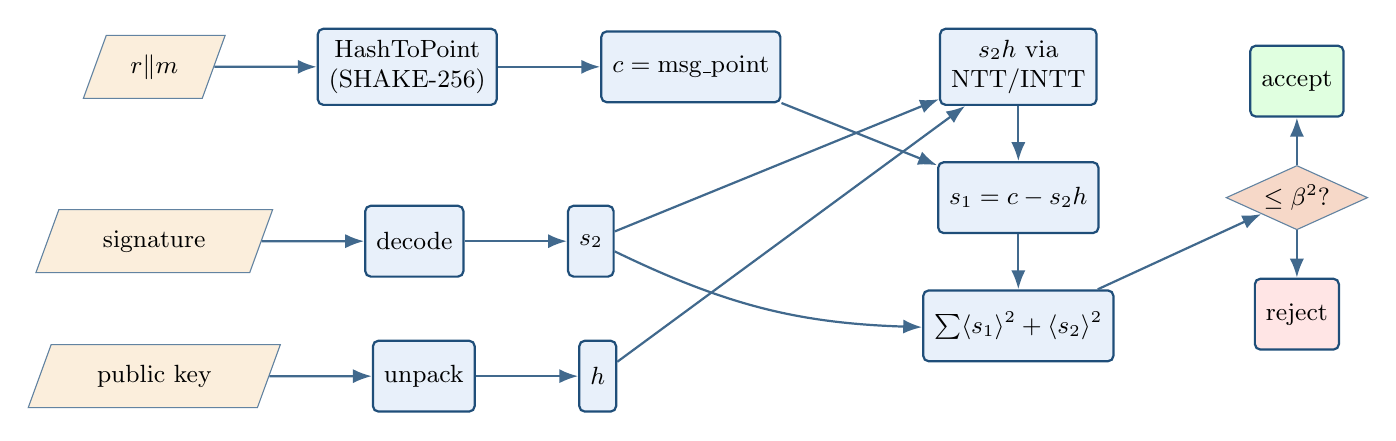
\begin{tikzpicture}[node distance=7mm and 13mm]
  \node[io] (msg) {$r\Vert m$};
  \node[proc, right=of msg] (h2p) {$\HtP$\\(SHAKE-256)};
  \node[proc, right=of h2p] (c) {$c=\text{msg\_point}$};

  \node[io, below=14mm of msg] (sig) {signature};
  \node[proc, right=of sig] (dec) {decode};
  \node[proc, right=of dec] (s2) {$s_2$};

  \node[io, below=9mm of sig] (pk) {public key};
  \node[proc, right=of pk] (decpk) {unpack};
  \node[proc, right=of decpk] (h) {$h$};

  \node[proc, right=20mm of c] (mul) {$s_2h$ via \\ $\NTT/\INTT$};
  \node[proc, below=7mm of mul] (s1) {$s_1=c-s_2h$};
  \node[proc, below=7mm of s1] (norm) {$\sum\langle s_1\rangle^2+\langle s_2\rangle^2$};
  \node[dec, right=16mm of s1] (test) {$\le\beta^2$?};
  \node[proc, above=6mm of test, fill=green!12] (acc) {accept};
  \node[proc, below=6mm of test, fill=red!10] (rej) {reject};

  \draw[arr] (msg)--(h2p); \draw[arr] (h2p)--(c);
  \draw[arr] (sig)--(dec); \draw[arr] (dec)--(s2);
  \draw[arr] (pk)--(decpk); \draw[arr] (decpk)--(h);
  \draw[arr] (s2) -- (mul); \draw[arr] (h) -- (mul);
  \draw[arr] (c) -- (s1); \draw[arr] (mul) -- (s1);
  \draw[arr] (s1) -- (norm); \draw[arr] (s2) to[bend right=12] (norm);
  \draw[arr] (norm) -- (test);
  \draw[arr] (test) -- (acc); \draw[arr] (test) -- (rej);
\end{tikzpicture}
\caption{On-chain verification pipeline. Hash-to-point may be precomputed off-chain
(FN-DSA interop path), in which case $c$ arrives in the signature payload.}
\label{fig:verify}
\end{figure}

% ===========================================================================
\section{Code-generation pipeline}
The unrolled NTT is not hand-written: a Rust circuit DSL traces the transform, validates it by
replay, and emits Cairo. Figure~\ref{fig:codegen} shows the flow; the same op-trace is checked
against an integer reference before emission (the correctness oracle).

\begin{figure}[h]
\centering
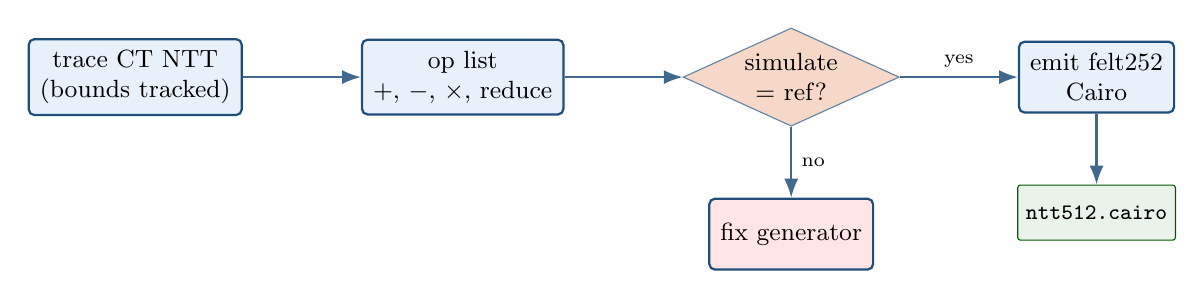
\begin{tikzpicture}[node distance=6mm and 15mm]
  \node[proc] (trace) {trace CT NTT\\(bounds tracked)};
  \node[proc, right=of trace] (ops) {op list\\ $+$, $-$, $\times$, reduce};
  \node[dec, right=of ops] (sim) {simulate\\ $=$ ref?};
  \node[proc, right=of sim] (emit) {emit felt252\\ Cairo};
  \node[file, below=9mm of emit] (out) {ntt512.cairo};
  \node[proc, below=9mm of sim, fill=red!10] (fix) {fix generator};

  \draw[arr] (trace)--(ops); \draw[arr] (ops)--(sim);
  \draw[arr] (sim)-- node[above,font=\scriptsize]{yes} (emit);
  \draw[arr] (sim)-- node[right,font=\scriptsize]{no} (fix);
  \draw[arr] (emit)--(out);
\end{tikzpicture}
\caption{Code generation: bounds-tracking trace $\to$ simulate oracle $\to$ emit. The
generator is a strongly-typed replacement for a Python DSL and shares constants with the Rust
reference.}
\label{fig:codegen}
\end{figure}

% ===========================================================================
\section{Optimization}\label{sec:opt}

\subsection{Typed bounds and \texttt{felt252} mode}
Representing coefficients as $\texttt{BoundedInt}\langle0,q{-}1\rangle$ lets the compiler prove
the absence of overflow, eliminating runtime range checks. When all intermediates provably stay
below $2^{128}$, the generator switches to native \texttt{felt252} arithmetic and reduces only
where necessary---cutting the generated NTT from $\sim$41.6k lines (typed) to $\sim$11.3k.

\subsection{Lazy reduction and the shift trick}
A butterfly \eqref{eq:butterfly} roughly multiplies the magnitude bound by $q$. After $\ell$
unreduced layers,
\begin{equation}
  |\text{value}| \;\le\; (q-1)\,q^{\ell}.
\end{equation}
Reducing every $6$ layers keeps this below $q^{7}\approx 2^{95} < 2^{128}$, so a \texttt{felt}
value maps faithfully to \texttt{u128} and reduction is a single $\bmod\,q$. Subtraction is
kept non-negative in the field by adding a shift: for $a-b$ with $b\in[0,B]$,
\begin{equation}
  a - b \;\equiv\; a + \Delta - b \pmod q,\qquad \Delta = q\bigl\lceil B/q\bigr\rceil \ge B,
\end{equation}
so the emitted expression never underflows into a large field element.

\subsection{Unrolled vs.\ looped, and compiler limits}
The fully-unrolled NTT is fast but large; two copies (verify needs two transforms) exceed the
Sierra compiler's per-function offset limit and its statement-count cast bound under the test
runner. The mitigations, in order of effect: (i) chunk the transform into per-layer functions;
(ii) run the full two-NTT verifier through \texttt{scarb cairo-run} (a different compilation
path); (iii) for an audit-friendly baseline, use a \emph{looped} NTT---correct and small, but
markedly slower. These occupy different points on the cost/compilability frontier.

\subsection{Hash choice}
Hash-to-point dominates cost. Measured per Keccak-$f[1600]$ permutation in pure Cairo versus
the Poseidon builtin:
\begin{center}
\begin{tabular}{lrr}
\toprule
per permutation & steps & L2 gas \\
\midrule
Poseidon (builtin) & $\sim$36 & $\sim$3.9k \\
Keccak-$f[1600]$ (pure Cairo) & $\sim$360{,}000 & $\sim$50\,M \\
\bottomrule
\end{tabular}
\end{center}
Standard SHAKE-256 hash-to-point ($\sim$10 permutations) is therefore $\sim$3.7\,M steps---the
reason a Poseidon variant is $\sim$50$\times$ cheaper but non-interoperable. A future
\texttt{keccak\_f1600} syscall (SNIP-32) would collapse the gap.

% ===========================================================================
\section{Measured results}
\begin{center}
\begin{tabular}{lrr}
\toprule
Component (Falcon-512) & steps & L2 gas \\
\midrule
$\Zq$ op & $\sim$60 & $\sim$40k \\
Unrolled $\NTT$-512 (felt252, lazy reduce) & 57{,}005 & 17.2\,M \\
SHAKE-256 hash-to-point (pure Cairo) & 3{,}727{,}918 & 534\,M \\
Hint-based verify (two NTTs $+$ norm, cairo-run) & 143{,}557 & --- \\
Direct-NTT verify (looped port) & 1{,}094{,}283 & 125.8\,M \\
Norm acceptance bound $\lfloor\beta^2\rfloor$ & \multicolumn{2}{r}{$34{,}034{,}726$} \\
\bottomrule
\end{tabular}
\end{center}
The unrolled/hint path fits a transaction budget; the looped/direct path is audit-friendly but
exceeds it---quantifying the trade the design must make.

\end{document}
